\chapter{Introduction} \label{chap:intro}
This work is focused on the linear optics and coupling studies and corrections applied during the commissioning of the Sirius storage ring. Sirius is the new Brazilian 4\ts{th} generation synchrotron light source with low emittance. In this chapter the general concepts and terminology regarding synchrotron light sources will be introduced in the Section~\ref{sec:sls}. The main information about the Sirius project will be presented in Section~\ref{sec:sirius_project}. To conclude the chapter, a scientific background related to the studies realized in this work is discussed and the master's goals are exhibited in the final section.
\section{Synchrotron Light Sources}\label{sec:sls}
Charged particles in relativistic speed radiates synchrotron light when accelerated~\cite{jackson}. The synchrotron light sources are scientific facilities where this effect is ultimately exploited in order to produce synchrotron light with high brightness and a broad energy range, with a spectrum covering from infrared light up to hard X-rays. The synchrotron light sources are high quality and versatile scientific tools that allow for a great diversity of high resolution experiments in several research areas, such as materials sciences, condensed matter physics, nanotechnology and many other areas.

Generally a synchrotron light source is composed by three main components: the injection system, the storage ring and the beamlines. Typically the charged particles used in these facilities are electrons. A brief description of each subsystem can be made:
\begin{description}[align=left]
    \item[Injection system:] composed by a \gls{linac} and a Booster. The electrons are emitted from an electron gun and accelerated by \gls{rf} structures in the \gls{linac}. Then the electrons are injected in the first circular accelerator, the Booster, where the energy ramp is performed from the low energy obtained at the end of \gls{linac} until the high operation energy in the storage ring.
    \item[Storage ring:] after the extraction from the Booster ring, the ultra-relativistic electrons are injected in the second circular accelerator, the storage ring, where electromagnetic fields are used to confine the electrons in stable closed orbits for many hours. In this approximated circular orbits the electrons produce the synchrotron light that is supplied to the beamlines.
    \item[Beamlines:] experimental stations installed tangentially to the storage ring, where the synchrotron light produced is used in a wide variety of scientific studies based on the radiation-matter interactions.
\end{description}

Typical values for the ``low'' energy obtained in the \gls{linac} are hundreds of \si{\mega\electronvolt} and the high nominal energy in the storage ring are few \si{\giga\electronvolt}. The whole injection process occurs with a repetition rate of a few \si{\hertz} until the storage ring is filled with electrons, reaching the operation current. The injection event might occur only in specific times of the day and in this case the storage ring operates in the so-called decay mode. The injection system may also fill the storage ring more frequently to keep the stored current almost constant during operation, this is called top-up mode.

The quality of the radiation produced in synchrotron light sources can be measured by the quantity called brightness. It is a measurement of the radiation intensity and collimation for a given energy and can be defined as:
\begin{equation}
    B(\omega) = \dfrac{F(\omega)}{\Sigma_x \Sigma_{x'} \Sigma_y \Sigma_{y'} \left(\Delta \omega /\omega\right)}.
\end{equation}

The photon frequency $\omega$ is related to the photon energy by $E = \hbar \omega$. The photon flux is represented by $F(\omega)$ and it is the average of the number of photons per second. The products $\Sigma_x \Sigma_{x'}$ and $\Sigma_y\Sigma_{y'}$ are the photon beam volumes in the horizontal and vertical phase space, respectively. The frequency bandwidth $\Delta \omega/\omega$ considered in the brightness calculation is typically $0.1\%$. The photon beam volume in phase space depends both on the photon and the electron distributions. The electron beam volume in the phase space is called beam emittance and it is a property derived from the storage ring magnetic lattice configuration. 

In order to achieve high brilliance for a synchrotron light source, one must increase the photon flux by increasing the electron energy and current and also minimizing the electron beam emittance. Reducing the electron beam emittance is equivalent to reduce the electron beam size and divergence. Constant advances both in the theoretical and technological aspects has been made in the accelerator community in the last decades, allowing for tremendous gains in the brightness of synchrotron light sources. 

Such great increments in the brightness scales have made it possible to classify the synchrotron light sources in generations. The 1\ts{st} synchrotron light source generation appeared as a parasitic effect from the bending magnets in particle colliders. The 2\ts{nd} generation were dedicated light sources built for the production of synchrotron radiation, generated mainly by bending magnets. The 3\ts{th} generation light sources were optimized to produce synchrotron radiation with \glspl{id} installed in long straight sections (originally without magnets) in the storage ring. The \glspl{id} are arrays of magnetic blocks organized in an alternated manner such that the electron beam follows a transversely undulating path when it passes through the device. The sequence of transverse accelerations induce the electrons to radiate synchrotron light, which may interfere to produce a photon beam with very high intensity and a sharp spectrum, as compared to the light emitted at the dipoles. Depending on the magnetic fields in the \gls{id}, the polarization of the emitted radiation can also be varied. The \glspl{id} used in 3\ts{th} synchrotrons are wigglers and undulators.

In the 4\ts{th} (and currently the newest) generation of synchrotron light source, recent developments in the accelerator field has been applied to reduce the electron beam emittance by orders of magnitude as compared to the previous generation. The 4\ts{th} generation is also known as \glspl{dlsr} based light sources. Undulators are also used as \glspl{id} in the storage ring long straight sections. Presently, these modern storage rings deliver synchrotron light to the beamlines with the highest brightness and coherence flux ever achieved in the history of synchrotron light sources. A brief overview about the main ideas applied in the \glspl{dlsr} will be given in the Subsection~\ref{subsec:fourth_generation}.
\subsection{Main Devices in a Storage Ring}


\begin{description}
    \item[Dipoles:]
    \item[Quadrupoles:]
    \item[Sextupoles:]
    \item[Correctors:]
    \item[\glspl{bpm}:]
\end{description}

\begin{figure}
\centering
%        \setlength\belowcaptionskip{-1.5ex}
\begin{subfigure}[t]{0.32\textwidth}
\includegraphics[width=0.9\textwidth]{figures/dipole_example.png}
    \caption{Dipole}
    \label{fig:nperiodic1}
\end{subfigure}
 \begin{subfigure}[t]{0.32\textwidth}
\includegraphics[width=1.0\textwidth]{figures/quadrupole_example.png}
    \caption{Quadrupole}
    \label{fig:nperiodic2}
\end{subfigure}
 \begin{subfigure}[t]{0.32\textwidth}
    \includegraphics[width=1.08\textwidth]{figures/sextupole_example.png}
    \caption{Sextupole}
    \label{fig:npdiflog}
\end{subfigure}
\caption{Schematic examples of magnets types used in storage rings.}
\label{fig:subfigures}
\end{figure}
\subsection{Fourth Generation Light Sources}\label{subsec:fourth_generation}


\section{The Sirius Project}\label{sec:sirius_project}
\subsection{Basic Parameters}
\begin{table}
        \centering
        \caption{Main Parameters of the Sirius Storage Ring.}
        \label{tab:sirius_main_parameters}
        \begin{tabular}{lccccl}
            \mr{2}{*}{Parameter} &  \mr{2}{*}{Symbol} & \mc{3}{c}{Operation Phases}& \mr{2}{*}{Unit}\\\cmidrule{3-5}
                                 &                    &Commiss. & Phase 1 & Phase 2& \\\toprule\toprule
            Energy               & $E_0$     & \mc{3}{c}{3.0}    & \si{\giga\electronvolt}\\
            Gamma factor         & $\gamma$  & \mc{3}{c}{5871}& \\
            Circumference        & $L_0$     & \mc{3}{c}{518.396}  & \si{\meter}\\
            Revolution period    & $T_0$     & \mc{3}{c}{1.729}   & \si{\micro\second}\\
            Revolution frequency & $f_0$     & \mc{3}{c}{578}    & \si{\kilo\hertz}\\
            Harmonic number      & $h$       & \mc{3}{c}{864}    & \\
            Momentum compaction  & $\alpha$  & \mc{3}{c}{\SI{1.636e-4}{}}& \\
            Transverse tunes (H/V)& $\nu_{x/y}$   & \mc{3}{c}{49.096/14.152}  & \\
            Energy loss per turn & $U_0$     & \mc{3}{c}{473}    & \si{\kilo\electronvolt} \\
            Natural emittance    & $\varepsilon_0$& \mc{3}{c}{251}& \si{\pico\meter\radian} \\
            Natural energy spread& $\sigma_\delta$& \mc{3}{c}{\SI{8.5e-4}}& \\\midrule
            % Damping times (H/V/L)& $\tau_{x/y/z}$ & \mc{3}{c}{16.9/22.0/12.9}& \si{\milli\second}\\
            % Damping rates (H/V/L)& $\alpha_{x/y/z}$ & \mc{3}{c}{59.5/45.8/77.8}& \si{\hertz}\\\midrule
            Nominal total current& $I_0$     & 30    &  100  & 350 & \si{\milli\ampere}\\
            RF cavity            &  & 1 7-Cell & \mc{2}{c}{2 SC-RF}  \\
            Voltage gap          & $V_0$     & 1.8   & \mc{2}{c}{3.0}& \si{\mega\volt} \\
            Natural bunch length & $\sigma_z$& 3.2(10.7) & \mc{2}{c}{2.5(8.2)}& \si{\milli\meter} (\si{\pico\second}) \\
            Synchrotron Tune     & $\nu_z$& \SI{3.56e-3} & \mc{2}{c}{\SI{4.6e-3}}& \\\bottomrule\bottomrule
        \end{tabular}
    \end{table}

\subsection{Magnetic Lattice and Linear Optics}
\begin{figure}
    \centering
    \includegraphics[scale=0.5]{figures/sirius_building.jpg}
    \caption{Sirius building layout~\cite{wiki}.}
    \label{fig:sirius_building}
\end{figure}
\begin{figure}
    \centering
    \includegraphics[scale=0.23, trim={0 2cm 0 0}, clip]{figures/sirius_lattice.png}
    \caption{Sirius 5BA magnetic lattice cells. The magnets are represented by colored blocks. Dipoles (B) are in blue, quadrupoles (Q) in orange and sextupole (S) in green. The cells are characterized by their straight sections types: high-beta (A) or low-beta (B, P). The Sirius storage ring is composed by 5 super-periods, each one composed by the four cells sequence A-B-P-B~\cite{wiki}.}
    \label{fig:sirius_lattice}
\end{figure}
\begin{figure}
    \centering
    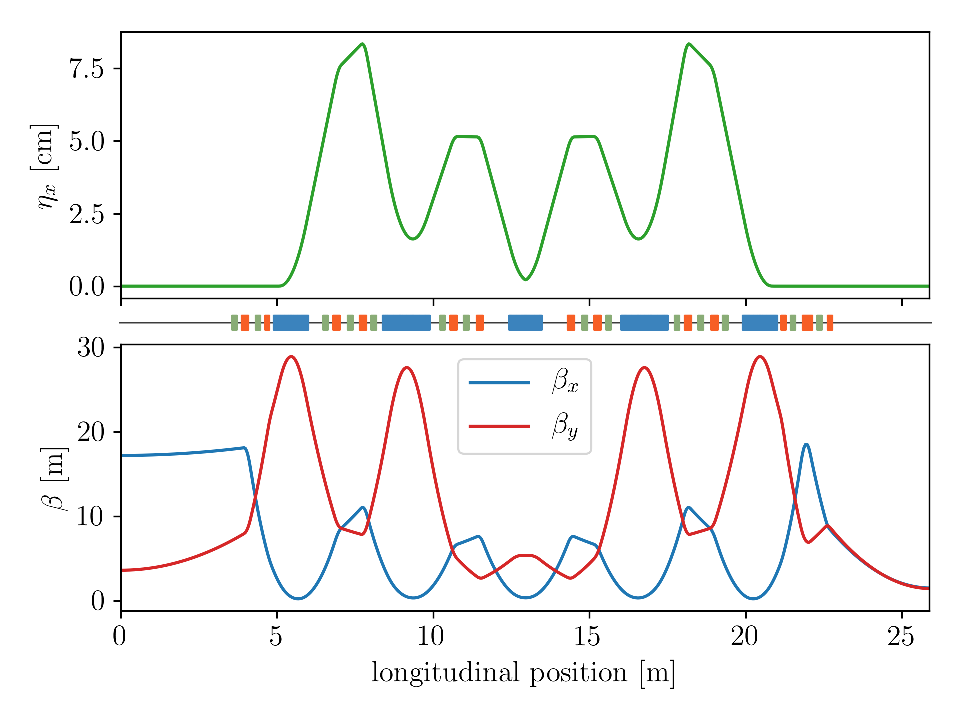
\includegraphics[scale=1.0]{figures/twiss_plot_refine.eps}
    \caption{Lattice functions for one 5BA cell for the Sirius storage ring with a high-beta straight section in the left and a low-beta in the right.}
    \label{fig:twiss_functions}
\end{figure}

\subsection{Comissioning}
\section{Scientific Background}
\section{Master's Objectives}






